\documentclass[a4paper]{article}

\usepackage{amsmath}
\usepackage{listings}
\usepackage{amsfonts}
\usepackage{amssymb}
\usepackage{graphicx}
\usepackage{titling}
\usepackage[utf8]{inputenc}
\usepackage[english]{babel}
\usepackage{fancyhdr}
\usepackage{lastpage}
\usepackage{textcomp}
\usepackage{hyperref}
\usepackage{float}
\usepackage{color, soul}

\addtolength{\oddsidemargin}{-.875in}
\addtolength{\evensidemargin}{-.875in}
\addtolength{\textwidth}{1.75in}
\addtolength{\topmargin}{-.875in}
\addtolength{\textheight}{1.75in}

\title{\Huge Medical Technologies Synopsis \vspace{1cm}}
\author{MrRattoSpaccio, Lolinear}
\date{May 23rd 2019}
\setcounter{page}{0}
\pagestyle{fancy}
\fancyhf{}

\fancyfoot[C]{Page \thepage \hspace{1pt} of \pageref{LastPage}}

\begin{document}
\maketitle
\thispagestyle{empty}
\pagebreak
\tableofcontents
\pagebreak
\section{Introduction}
\subsection{Tipologie di Ingegneri biomedici}
\begin{description}
    \item[Clinici] Lavorano negli ospedali, essi aiutano altri operatori degli
    ospedali a scegliere l'apparecchiatura più giusta per l'assistenza ai 
    pazienti. Si occupano anche di assicurare che le apparecchiature siano
    sicure ed affidabili.
    \item[Progetto e Ricerca] Lavorano nelle grandi aziente, progettano sistemi
    per il monitoraggio continuo dei pazienti critici, organi artificiali, o 
    schemi e procedure per somministrare terapie in modo sicuro ed efficace.ù
    \item[Riabilitazione] Utilizzano la tecnologia ed i calcolatori per 
    aiutare le persone con disabilità e migliorare la qualità della loro vita.
    \item[Ricerca (Scuole)] Lavorano nei laboratori di ricerca di scuole di 
    medicina o università, acquisendo nuove conoscenze sugli organismi viventi.
    \item[Vari] Alcuni studiano cellule ed insiemi di molecole, alcuni organi
    composti da insiemi di cellule, altri creano modelli matematici che 
    descrivono le funzionalità del corpo. Altri ancora studiano materiali
    artificiali necessari alla creazione di dispositivi medicali. 
\end{description}
\subsection{Dispositivi medicali (DM)}
\subsubsection{Definizione}
\paragraph{Completa}
S’intende per dispositivo medicale, qualunque strumento, apparecchio, 
apparecchiatura, materiale, prodotto, all’eccezione dei prodotti d’origine 
umana, o altro articolo usato da solo o in combinazione, compresi gli accessori
e software necessari per il suo funzionamento, destinato dal fabbricante ad 
essere impiegato sull'uomo per scopi medici e la cui azione principale voluta 
non si ottiene con mezzi farmacologici o immunologici o metabolici, ma dove 
la funzione può essere assistita da tali mezzi.
\paragraph{Concisa}
Ogni prodotto utilizzato per scopi medici che non è, né un medicamento, né un 
prodotto biologico, è identificabile con la terminologia di Dispositivo Medico.
\subsubsection{Utilizzi}
\begin{itemize}
    \item Diagnosi, prevenzione, controllo, terapia o attenuazione di una 
    malattia
    \item Diagnosi, controllo, terapia, attenuazione o compensazione di una 
    ferita o di un handicap
    \item Studio, sostituzione o modifica dell'anatomia o di un processo 
    fisiologico
    \item Controllo e gestione del concepimento
\end{itemize}
\subsubsection{Categorie}
\begin{description}
    \item[Impiantabili attivi (DMIA)] Pacemaker, defibrillatori, pompe 
    \item[Diagnostica in Vitro (DM DIV)] Reagenti per le diagnosi
    \item[Compensazione degli handicap] Sedia a rotelle, apparecchi acustici
    occhiali, ecc.
    \item[Su misura] protesi dentarie, plantari ortopedici, ecc.
    \item[Diagnostica/Pratiche Terapeutiche/Supporto Vitale] Scanner, macchina
    per la dialisi, radioterapia, monitor di sorveglianza, defibrillatori
    esterni
    \item[Monouso] Aghi, bende, siringe, ecc.
    \item[Impianti chirurgici non attivi] protesi d'anca, valvole cardiache, ecc.
\end{description}
\subsection{Dispositivi Medicali Impiantabili Attivi (DMIA)}
Dispositivi medici che sono progettati per essere impiantati totalmente o in 
parte nel corpo umano... e che dipendono per il loro corretto funzionamento 
da una fonte d’energia elettrica o da qualsiasi altra fonte d’energia diversa 
da quella prodotta direttamente dal corpo umano o dalla gravità.
\subsection{Dispositivi Medicali di Diagnostica In Vitro (DM DIV)}
Prodotti, reagenti, materiali, strumenti... destinati ad essere utilizzati in 
vitro per l'esame di campioni provenienti dal corpo umano con lo scopo di 
fornire informazioni relative a una condizione fisiologica o patologica.
\subsection{Classificazione dei DM}
I dispositivi medici, eccetto i DMIA e i DM DIV sono classificati in 4 classi:
\begin{itemize}
    \item Classe I $\to$ Rischio potenziale debole (Lenti da vista, 
    Stetoscopi, ecc.)
    \item Classe IIa $\to$ Rischio potenziale moderato (Lenti a contatto, 
    Catateri urinari, ecc.)
    \item Classe IIb $\to$ Rischio potenziale elevato (Laser chirurgici, 
    Cemento osseo, ecc.)
    \item Classe III $\to$ Rischio potenziale critico (Stent, valvole cardiache, 
    ecc.)
\end{itemize}
Tutti i DMIA sono classificati come Classe III.
\subsubsection{Regole di classificazione}
\begin{itemize}
\item Il periodo d’utilizzo o più precisamente la durata in cui il dispositivo
è in continuità in contatto col paziente
\item L’invasività: il dispositivo è invasivo o no, e se lo è, qual è il grado
d’invasività (penetrazione attraverso un orifizio del corpo o tramite 
impianto chirurgico)
\item La possibilità o meno di riutilizzo
\item L’obiettivo terapeutico o diagnostico
\item La dipendenza da una fonte d’alimentazione diversa da quella umana
\item La parte del corpo che viene a contatto con il dispositivo medico: sistema circolatorio centrale,
sistema nervoso centrale, ecc.
\end{itemize}
\paragraph{Classe I}
Strumenti chirurgici riutilizzabili, dispositivi medici non invasivi, 
dispositivi medici invasivi per uso temporaneo, ecc.
\paragraph{Classe IIa}
Dispositivi medici di classe I sterili e/o con funzione di misurazione, lenti a 
contatto, protesi dentarie, ecc.
\paragraph{Classe IIb}
Dispositivi medici impiantabili a lungo termine, ecc.
\paragraph{Classe III}
Dispositivi medici impiantabili a lungo termine in contatto con il cuore, il 
sistema circolatorio centrale o il sistema nervoso centrale, i dispositivi 
medici impiantabili riassorbibili, protesi al seno, protesi d'anca, protesi
di ginocchio, ecc.
\subsection{Prodotti di Frontiera}
Si parla di prodotti combinati o di frontiera:
\begin{itemize}
    \item Quando un DM forma con un farmaco un prodotto un prodotto integrato.
    Ad esempio le siringhe pre-riempite.
    \item Quando un DM incorpora una sostanza che, utilizzata sola, può essere
    considerata come un farmaco. Ad esempio il cemento osseo con antibiotico.
\end{itemize}
Il prodotto combinato è considerato come un farmaco o un dispositivo medico in 
base all'azione principiale prevista.
\subsection{Considerazioni e Prospettive nel campo}
Troppo spesso l'utilizzo delle tecnologie medicali o viene promosso con
eccessiva facilità senza averne valutato adeguatamente le implicazioni o viene 
limitato dai timori derivanti dall’incertezza circa gli esiti e le conseguenze
del loro impiego. \\
La figura tecnica di riferimento per le tecnologie sanitarie, quale l’ingegnere 
biomedico, deve compiere uno sforzo di ampliamento del suo background formativo
e focalizzare maggiore attenzione sugli aspetti di valutazione dei rischi, dei 
costi e dei benefici delle nuove tecnologie sanitarie.

\section{Organizzazione del corpo umano, cellule e tessuti}
\paragraph{Anatomia} La scienza che studia la struttura di un corpo e le 
relazioni tra le sue parti.
\paragraph{Fisiologia} La scienza che studia come funzionano le parti di un
organismo.
\subsection{Livelli di organizzazione ed apparati del corpo}
\begin{enumerate}
    \item Livello della chimica (o molecolare): include gli atomi e le molecole
    \item Livello cellulare: le cellule sono le unità strutturali e funzionali 
    di base dell’organismo
    \item Livello dei tessuti: i tessuti sono costituiti da gruppi di cellule 
    che svolgono una funzione particolare
    \item Livello degli organi: i diversi tipi di tessuti si uniscono a formare 
    gli organi
    \item Livello dei sistemi e degli apparati: i sistemi sono costituiti da 
    organi con la medesima origine embriologica; gli apparati possono avere 
    struttura o derivazione embriologica diversa
    \item Livello dell’organismo
\end{enumerate}
\begin{figure}[H]
    \centering
    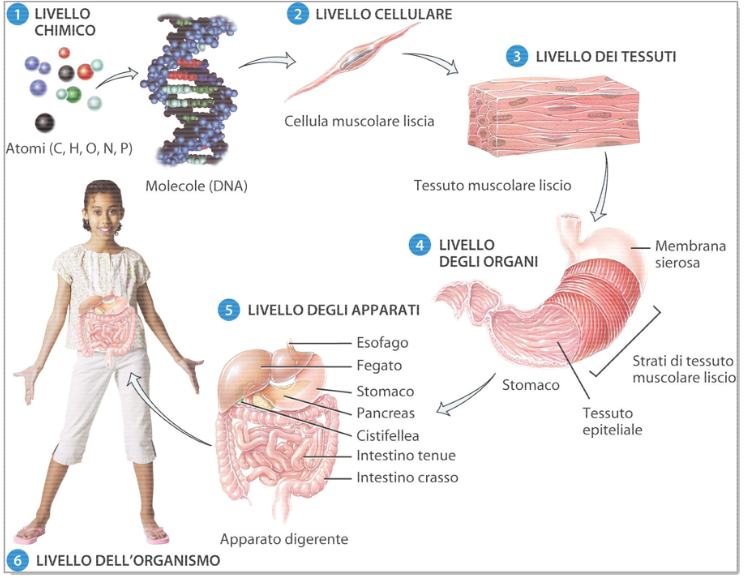
\includegraphics[scale=0.3]{figures/levels.png}
    \caption{Livelli di organizzazione}
\end{figure}
\subsection{Processi della vita}
\begin{description}
    \item[Metabolismo] L'insieme di tutti i processi chimici che avvengono nel
    corpo, tra cui la scissione di molecole e la loro sintesi
    \item[Reattività] La capacità di rilevare e di rispondere ai cambiamenti
    dell'ambiente interno/esterno
    \item[Movimento] Gli spostamenti di tutto il corpo, compresi gli organi, le
    cellule e gli organuli cellulari
    \item[Accrescimento] L'aumento delle dimensioni corporee
    \item[Differenziazione] Il processo in cui le celle indifferenziate si
    specializzano
    \item[Riproduzione] Intesa come sintesi di nuove cellule e generazione di
    un nuovo individuo
\end{description}
\subsection{Omeostasi}
L'omeostasi è il mantenimento della stabilità delle condizioni del corpo. 
Essa:
\begin{itemize}
    \item Garantisce il funzionamento cellulare
    \item Interviene per ripristinare le condizioni di stabilità 
    controbilanciando i cambiamenti interni/esterni
    \item Varia entro un ristretto ambito compatibile coi processi vitali delle
    cellule
\end{itemize}
Esistono dei sistemi di feed-back che permettono il mantenimento dell'omeostasi,
rappresentati da un ciclo di eventi dove la condizione del corpo viene 
continuamente monitorata, valutata e modificata. Così facendo si ottiene una
condizione controllata, perturbabile da uno \textbf{stimolo}.

\subsubsection{Sistemi di feed-back}
Un sistema di feed-back è costituito da:
\begin{description}
    \item[Recettore] Struttura che rileva i cambiamenti che avvengono in una 
    condizione controllata e invia tale informazione o input a un centro di 
    controllo
    \item[Centro di controllo] Valuta l’input ricevuto e invia comandi in 
    uscita all’effettore per il ripristino della condizione controllata
    \item[Effettore] Struttura che riceve l’output e produce una risposta 
    che modifica la condizione controllata
\end{description}
Possono essere di due tipologie:
\begin{description}
    \item[Retroazione positiva] Se il cambiamento prodotto in una condizione
    controllata viene rafforzato
    \item[Retroazione negativa] Se il cambiamento prodotto in una condizione
    controllata viene invertito
\end{description}
Nel caso di uno squilibrio dell'omeostasi si identifica come \textbf{disturbo}
una qualsiasi deviazione dalla norma riscontrabile in una struttura/funzione.
Se un \textit{disturbo} è contraddistinto da sintomi e segnali riconoscibili,
viene definito come \textbf{malattia}.
\subsection{Suddivisione del corpo}
Il corpo umano è diviso convenzionalmente in:
\begin{itemize}
    \item Testa
    \item Collo
    \item Tronco
    \item Arti superiori
    \item Arti inferiori
\end{itemize}
I termini di posizione vengono usati per descrivere la posizione di una parte 
rispetto a un’altra. \\
Le parti del corpo sono divise in 4 \textbf{piani} principali:
\begin{figure}[H]
    \centering
    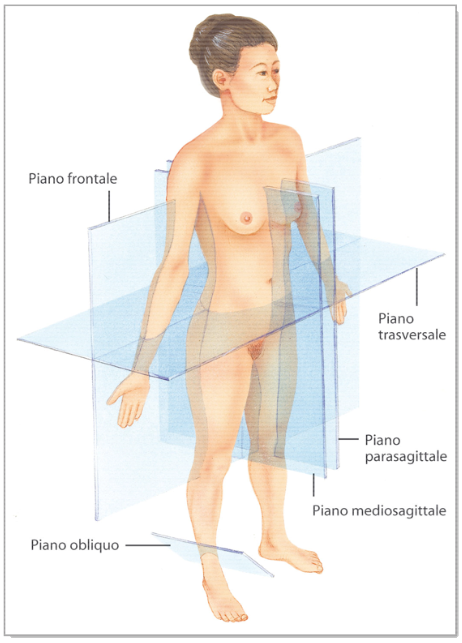
\includegraphics[scale=0.3]{figures/planes.png}
    \caption{Piani del corpo}
\end{figure}
\noindent
Gli spazi interni al corpo che contengono, proteggono, separano e sostengono
gli organi sono definiti come \textbf{cavità corporee} e si suddividono in:
\begin{figure}[H]
    \centering
    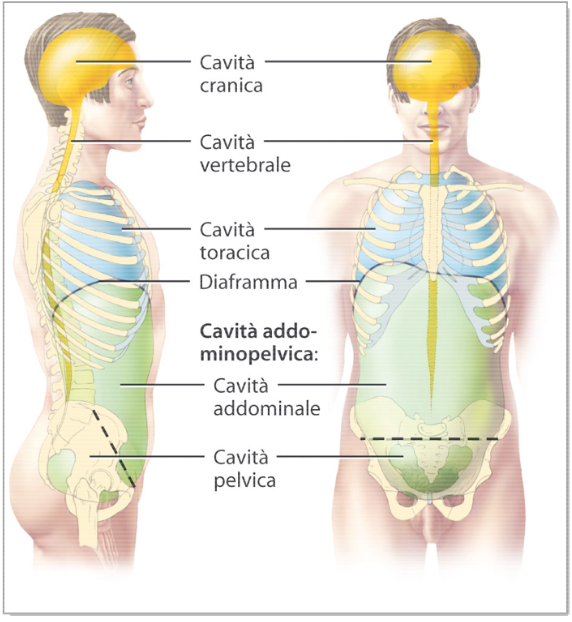
\includegraphics[scale=0.3]{figures/holes.png}
    \caption{Cavità corporee}
\end{figure}
\subsection{Chimica del corpo umano}
\begin{description}
\item[Ione] Un atomo che abbia ceduto o acquistato uno o più elettroni
\item[Molecola] Combinazione di due o più atomi che condividono i propri 
elettroni
\item[Composto] Sostanza contenente atomi di due o più elementi diversi
\item[Radicale libero] Ione o molecola dotato di carica con un elettrone 
spaiato nel guscio più esterno
\item[Energia chimica] Forma di energia utilizzabile immagazzinata 
nei legami delle molecole
\item[Anabolismo] Reazioni di sintesi che avvengono all’interno del corpo
\item[Catabolismo] Reazioni di scomposizione che hanno luogo nell’organismo
\item[Metabolismo] Anabolismo e catabolismo vengono indicati con il termine 
di metabolismo
\item[Acido] Sostanza che sciogliendosi in acqua rilascia uno o più ioni 
idrogeno (H)
\item[Base] Sostanza che sciogliendosi in acqua rilascia uno o più ioni 
idrossido (OH)
\end{description}
Acidi e basi reagiscono tra loro a formare i \textbf{sali}. I sali, sciolti 
nell’acqua, si scindono in \textbf{cationi} e \textbf{anioni}. \\ \\
I \textbf{composti inorganici} sono generalmente privi di carbonio, con 
struttura semplice e sono uniti da legami ionici e covalenti. \\ \\
I \textbf{composti organici} contengono sempre carbonio, spesso idrogeno e 
hanno sempre legami covalenti.
\subsection{Composti organici nei processi della vita}
I principali composti organici sono:
\begin{itemize}
\item Carboidrati
\item Lipidi
\item Proteine
\item Acidi nucleici
\item ATP
\end{itemize}
\subsubsection{Carboidrati}
I carboidrati in base alla struttura si distinguono in monosaccaridi, 
disaccaridi, polisaccaridi.
\subsubsection{Lipidi}
I lipidi contengono sempre carbonio, idrogeno e ossigeno, ma hanno meno legami 
covalenti polari rispetto ai carboidrati. Si distinguono in trigliceridi 
(grassi e oli), fosfolipidi, steroidi.
\subsubsection{Proteine}
Le proteine sono macromolecole contenenti carbonio, idrogeno, ossigeno e 
azoto. I suoi monomeri sono definiti come \textbf{amminoacidi} e hanno un
gruppo amminico (-NH 2) e uno carbossilico (-COOH).
\subsubsection{Acidi nucleici}
\textbf{DNA} e \textbf{RNA}. Sono macromolecole contenenti carbonio, idrogeno, 
ossigeno, azoto e fosforo. I loro monomeri si chiamano \textbf{nucleotidi}. \\
Ogni nucleotide del DNA è composto da:
\begin{itemize}
    \item Una base azotata (A,C,G,T)
    \item Uno zucchero
    \item Un gruppo fosfato
\end{itemize}
L'RNA è invece composto da: 
\begin{itemize}
    \item Una base azotata (A,C,G,U)
    \item Zucchero ribosio
\end{itemize}
\subsubsection{ATP}
È la molecola usata per trasferire energia dalle cellule.
\subsection{Enzimi}
Gli enzimi sono proteine utilizzate dalle cellule per accelerare e ottimizzare 
le reazioni che avvengono al loro interno. Hanno tre caratteristiche:
\begin{description}
\item[Specificità] Ogni enzima catalizza (cioè orienta e accelera) una 
determinata reazione che coinvolge specifici substrati e dà origine a 
specifici prodotti.
\item[Efficienza] In condizioni ottimali un enzima può accelerare una reazione 
fino a miliardi di volte.
\item[Controllo] La velocità di sintesi e la concentrazione degli enzimi sono 
costantemente monitorate dai geni della cellula.
\end{description}
\subsection{Cellula}
La cellula è l’unità strutturale e funzionale fondamentale del corpo. È
composta da tre parti:
\begin{description}
\item[Membrana plasmatica] Costituisce e delimita la superficie esterna della 
cellula, separa l’interno dall’esterno.
\item[Citoplasma] È contenuto fra la membrana citoplasmatica e il nucleo. 
La porzione fluida è detta \textbf{citosol} ed al suo interno sono presenti 
vari tipi di organuli.
\item[Nucleo] È l’organulo più grande della cellula e agisce da centro di 
controllo.
\end{description}
\subsubsection{Membrana plasmatica} 
La membrana plasmatica è una barriera flessibile ma robusta costituita da un 
doppio strato fosfolipidico in cui sono parzialmente o interamente inserite 
delle proteine. È caratterizzata da permeabilità selettiva, meccanismo che 
consente il passaggio solo a determinate sostanze mentre lo impedisce ad altre.
\\ Le funzioni della membrana dipendono dal tipo di proteina:
\begin{description}
\item[Recettori] Riconoscono e legano una proteina specifica
\item[Enzimi] Per la catalisi di reazioni intra/extra-cellulari
\item[Riconoscimento] Identificano altre proteine o agenti estranei
\end{description}
Gran parte del nostro organismo è costituito da fluido intracellulare e 
fluido extracellulare. Il primo è contenuto all’interno delle cellule (citosol)
mentre l'altro è presente negli spazi microscopici fra le cellule adiacenti e 
viene detto anche fluido interstiziale. \\
Il gradiente di concentrazione è la differenza di concentrazione tra due aree 
diverse. Se i soluti si muovono da una zona con concentrazione più bassa si 
muovono \textbf{secondo gradiente}, altrimenti \textbf{contro gradiente}.
\\ Se una sostanza attraversa la membrana secondo gradiente allora utilizza
solo la propria energia di movimento e viene definito attraversamento tramite
\textbf{processi passivi}. Se invece la attraversa contro gradiente viene
utilizzata l'energia cellulare, sotto forma di ATP per spingerla attraverso,
e viene definito attraversamento tramite \textbf{processi attivi}. \\
I processi passivi possono avvenire in tre modi diversi:
\begin{itemize}
    \item Diffusione semplice
    \item Diffusione facilitata
    \item Osmosi (movimento netto di molecole d’acqua attraverso una membrana 
    a permeabilità selettiva)
\end{itemize}
I processi attivi invece in due:
\begin{itemize}
    \item Trasporto attivo (l'energia data dalla scissione dell'ATP cambia la
    conformazione di una proteina di trasporto che permette il passaggio)
    \item Trasporto con vescicole (le vescicole formatesi per gemmazione
    raccolgono le sostanze dal fluido cellulare e lo fanno passare, dentro
    $\to$ fuori è esocitosi, opposto endocitosi)
\end{itemize}
\subsubsection{Citoplasma}
Il citosol è la parte fluida del citoplasma e circonda gli organuli, è 
costituito da acqua (75-90\%), soluti e particelle sospese. Gli organuli sono
strutture specializzate interne alla cellula in cui avvengono processi
specifici. Gli organuli principali sono:
\begin{description}
\item[Citoscheletro] È una rete complessa di tre tipi di filamenti proteici 
che si estende per tutto il citosol
\item[Centrosoma] È una struttura posta vicino al nucleo e da cui prende avvio 
la divisione cellulare
\item[Ciglia e flagelli] Sono estensioni della membrana cellulare, di diversa 
lunghezza, protese verso l’esterno della cellula con il compito di spostare 
liquidi e secrezioni (es. nel tratto respiratorio) oppure l’intera cellula
(es. negli spermatozoi)
\item[Ribosomi] Sono i centri di sintesi delle proteine e sono ricchi di acido 
ribonucleico (RNA)
\item[Reticolo endoplasmatico] È una rete di membrane ripiegate, estesa per 
tutto il citoplasma. Ci sono due tipi di reticoli endoplasmatici: il RE liscio 
(REL) e il RE ruvido (RER). RE ruvido (RER): si estende a partire dalla 
membrana nucleare; presenta un aspetto ruvido perché costellato di ribosomi, 
che operano la sintesi proteica di componenti della membrana plasmatica. RE 
liscio (REL): reticolo di tubuli membranosi del tutto lisci perché privi di 
ribosomi. Qui avviene la sintesi di acidi grassi e steroidi
\item[Apparato di Golgi] È un complesso di sacche membranose appiattite, dai 
bordi rigonfi, impilate una sull’altra, con il compito di modificare e 
immagazzinare le proteine secrete dai ribosomi del RER
\item[Lisosomi] Sono vescicole racchiuse in membrane che contengono enzimi in 
grado di scindere una grande varietà di molecole. Trasportano e liberano nel 
citosol i prodotti finali della digestione
\item[Perossisomi] Sono simili ai lisosomi ma di minori dimensioni; contengono 
numerosi enzimi in grado di ossidare (sottrarre atomi di idrogeno) svariate 
sostanze organiche, svolgendo così una funzione di detossificazione
\item[Proteasomi] Sono strutture cilindriche con il compito di distruggere le 
proteine inutili, danneggiate o difettose. Contengono enzimi che scindono le 
proteine in amminoacidi riutilizzabili
\item[Mitocondri] Sono considerati le centrali energetiche cellulari poiché in 
essi avviene la sintesi di ATP. Sono costituiti da due membrane strutturalmente 
simili a quella plasmatica: la più interna è ripiegata in creste, che 
racchiudono uno spazio centrale o matrice dove avvengono le reazioni di 
sintesi dell’ATP. \textit{\textbf{Mitochondria is the powerhouse of the cell.}}
\end{description}
\subsubsection{Nucleo}
Il nucleo è la struttura cellulare di maggiori dimensioni, di forma sferica o 
ovale, presente in tutte le cellule del corpo tranne nei globuli rossi maturi.
Al suo interno si trovano i nucleoli, corpi sferici costituiti da proteine e 
acidi nucleici (DNA e RNA), dove vengono sintetizzati i ribosomi. Il nucleo 
contiene i geni (costituiti da DNA) che immagazzinano le istruzioni per la 
sintesi proteica.
\subsection{Sintesi delle proteine}
L’informazione contenuta in una regione specifica del DNA viene trascritta e 
produce una molecola di RNA che si lega a un ribosoma. Qui, l’informazione 
viene tradotta in una sequenza specifica e univoca di amminoacidi da cui si 
otterrà una proteina. L’informazione è contenuta nel DNA in quattro diversi 
nucleotidi che si appaiano in sequenze di tre. Ogni tripletta codificherà 
per un determinato amminoacido. Durante la trascrizione l’informazione delle 
triplette di DNA viene copiata in una sequenza complementare di codoni in un
filamento di RNA. Ci sono tre tipi di RNA:
\begin{description}
\item[Messaggero (mRNA)] Dirige la sintesi proteica
\item[Ribosomiale (rRNA)] Si unisce alle proteine ribosomiali per costruire i 
ribosomi
\item[Transfer (tRNA)] Lega un amminoacido e lo porta sul ribosoma perché 
venga incorporato nella proteina in costruzione.
\end{description}
La traduzione è il processo in cui l'mRNA si associa ai ribosomi e converte
la sequenza di nucleotidi in una sequenza specifica di amminoacidi.
Avviene in diverse fasi:
\begin{enumerate}
    \item mRNA si lega alla subunità ribosomiale ed il tRNA iniziatore si lega
    al codone di start dell'mRNA
    \item tRNA ha alle estremità un amminoacido specifico ed una tripletta di 
    nucleotidi (anticodone) e si lega all'mRNA
    \item L'anticodone di un nuovo tRNA riconosce il codone complementare 
    sull'mRNA e vi si lega
    \item Si formano i legami peptidici tra amminoacidi adiacenti
    \item Un nuovo tRNA con il suo amminoacido si lega al codone successivo
    allungando la proteina
    \item La sintesi termina quando il ribosoma aggiunge un codone di stop
\end{enumerate}

\subsection{Ciclo cellulare e divisione cellulare somatica}
È l'insieme delle fasi che caratterizzando la vita di ogni cellula. Tranne le
cellule sessuali (gameti) le cellule del corpo vengono definite somatiche e 
subiscono la \textbf{divisione cellulare somatica}. Consiste nella duplicazione
del DNA, aumento delle dimensioni e divisione di cellula e nucleo. Tra una e 
l'altra c'è l'\textbf{interfase}, dove la cellula si comporta normalmente e si
prepara alla divisione. \\ 
La fase mitotica si divide in:
\begin{description}
\item[Mitosi] Divisione del nucleo
\item[Citodieresi] La divisione del citoplasma e di tutti gli organuli in due
cellule indipendente
\end{description}
La mitosi si divide in:
\begin{enumerate}
    \item Profase: formazione del fuso miotico nel nucleo che inizia a
    disgregarsi
    \item Metafase: le coppie di cromatidi si allineano lungo i tubuli del fuso
    \item Anafase: separazione dei cromatidi ai poli opposti della cellula
    \item Telofase: formazione di un nuovo involucro nucleare, disfacimento del 
    fuso mitotico
\end{enumerate}
\subsection{Tessuti}
\subsection{Tessuto epiteliale}
Ricopre la superficie del corpo; riveste le cavità del corpo e forma le 
ghiandole. Ne esistono due tipi: rivestimento, che copre o riveste varie parti
del corpo e ghiandolare, che è fatto da cellule altamente specializzate che 
svolgono attività di secrezione. \\
Quelli di rivestimeno vengono classificati in base al numero di strati e forma
delle cellule. Quelli ghiandolari hanno la funzione di secernere particolari
sostanze all'interno delle ghiandole. \\
Le ghiandole possono essere endocrine o esocrine.
\subsection{Tessuto Connettivo}
È uno dei tessuti più abbondanti dell’organismo e svolge svariate funzioni. \\
Ce ne sono cinque tipi:
\begin{itemize}
    \item Tessuto connettivo lasso
    \item Tessuto connettivo denso
    \item Cartilagine
    \item Tessuto connettivo osseo
    \item Tessuto connettivo liquido
\end{itemize}
\subsection{Tessuto Muscolare}
È costituito da cellule allungate dette fibre muscolari. \\
Si classifica in: 
\begin{itemize}
\item Tessuto muscolare scheletrico (unito alle ossa dello scheletro)
\item Tessuto muscolare cardiaco (forma le pareti del cuore)
\item Tessuto muscolare liscio (presente nelle pareti di strutture cave quali 
organi e vasi sanguigni)
\end{itemize}
\subsection{Tessuto Nervoso}
È costituito da due soli tipi di cellule:
\begin{itemize}
    \item Neuroni (sensibili a stimoli)
    \item Cellule gliali (supporto)
\end{itemize}
\subsection{Membrane del corpo}
Sono strati piani di tessuto flessibile che ricoprono o rivestono le varie 
superfici del corpo. \\
Ce ne sono tre tipi:
\begin{itemize}
    \item Mucosa
    \item Sierosa
    \item Sinoviale
\end{itemize}
\subsubsection{Mucosa}
Riveste le cavità interne degli organi che comunicano con l’esterno e secerne 
muco con funzione difensiva e protettiva.
\subsubsection{Sierosa}
Riveste le cavità degli organi che non comunicano con l’esterno ed è costituita
dai foglietti parietale e viscerale, che secernono il liquido sieroso che 
riduce l’attrito fra gli organi.
\subsubsection{Sinoviale}
Riveste le cavità di alcune articolazioni e non presenta strato epiteliale e 
secerne il liquido sinoviale che lubrifica le ossa a livello delle 
articolazioni, nutre la cartilagine e rimuove eventuali batteri.

\section{Aspetti socio-economici, leggi, e norme}
\subsection{Generalità e definizioni}
Definizione di \textbf{dispositivo medico}:
\begin{quote}
    \centering
    Uno strumento, un apparecchio, un impianto, una sostanza, o altro prodotto 
    usato da solo o in combinazione, compreso il software informatico impiegato 
    per il suo corretto funzionamento, e destinato dal fabbricante ad essere 
    impiegato nell'uomo a scopo di:
    \begin{itemize}
        \item diagnosi, prevenzione, controllo, terapia o attenuazione di una 
        malattia (tomografo)
        \item diagnosi, controllo, terapia, attenuazione o compensazione di 
        una ferita o di un handicap (filo per suture)
        \item studio, sostituzione o modifica dell'anatomia o di un processo 
        fisiologico (protesi)
        \item intervento sul concepimento (profilattico)
    \end{itemize}
    Un dispositivo medico non deve esercitare la sua azione principale nel o 
    sul corpo umano con mezzi farmacologici o immunologici, né mediante processo 
    metabolico, anche se la sua funzione può essere coadiuvata da tali mezzi. 
\end{quote}
Definizione di \textbf{malattia}:
\begin{quote}
    \centering
    \hl{Alterazione dello stato fisiologico e psicologico dell'organismo}, capace di 
    ridurre, \hl{modificare negativamente} o persino eliminare le funzionaità normali 
    del corpo. Il concetto di malattia deve essere inteso come status e condizione 
    \hl{potenzialmente reversibile} attraverso l'applicazione di una terapia; questa 
    caratteristica di reversibilità é alla base del dibattito, sempre aperto, sul 
    fatto che alcuni stati dell'organismo dovuti alla genetica, come ad esempio la 
    condizione di sterilità, non siano definibili come malattia.
\end{quote}
\subsection{Aspetti socio-economici}
Nella medicina moderna, il problema non sembra più essere solo la guarigione e il 
recupero da una malattia ma anche quello di intervenire in anticipo e in qualche 
modo affinché la malattia o il semplice malessere non abbia neanche la possibilità 
di manifestarsi.

Condizioni legate al normale decorso della vita dell'organismo (menopausa, vecchiaia), 
o alla condotta di vita della persona (stress da lavoro), sono diventate vere e proprie 
patologie, con farmaci, terapie e strumenti atti al trattamento dei sintomi. Questo non 
può che avere profondi riflessi sull'estensione dei compiti ch evengono affidati alla 
medicina, spesso sulla base delle sue stesse proposte.

\subsection{Leggi e norme}
Il marchio CE, secondo il "nuovo approccio", definisce delle direttive da rispettare per 
l'ottenimento di un marchio CE che permette il libero scambio dei prodotti all'interno 
di una comunità. Le direttive introducono il seguente concetto fondamentale: 
\begin{quote}
    \centering
    Il fabbricante ha il dovere di rendere i propri prodotti sicuri e deve poter 
    dismostrare di aver fatto tutto il possibile per rendere i prodotti sicuri per poter 
    meglio definire, dai punti di vista costruttivo e della sicurezza, il libero scambio 
    interno dei prodotti di fabbricazione.
\end{quote}
Le direttive sono atti comunitari che:
\begin{quote}
    \centering
    vincolano lo stato membro per quanto riguarda il risultato da raggiungere, salva 
    restando la competenza degli organi nazionali in merito alla forma ed ai mezzi con 
    i quali raggiungere tali risultati.
\end{quote}
Le direttive non sono direttamente obbligatorie e vincolanti negli stati membri, ma sono 
implementate dagli organi nazionali competenti.
\subsection{Direttiva-tipo}
Nel nuovo approccio, una direttiva-tipo é strutturata secondo i seguenti criteri:
\begin{description}
    \item[Campo di applicazione]: prodotti coperti, rischi da evitare
    \item[Clausola generale di immissione sul mercato]: responsabile della sicurezza del 
    prodotto e della sua immissione sul mercato (usualmente il fabbricante o l'importatore)
    \item[Elenco dei requisiti essenziali di sicurezza]: sufficientemente precisi da 
    permettere la costituzione di obbligihi sanzionabili dagli stati membri
    \item[Clausola di libera circolazione]: garantisce la libera circolazione del prodotto
    marcato CE ed é la "ricompensa" per tempo e risorse investite per la certificazione
    \item[Norme armonizzate]: riferimento alle norme tecniche e di sicurezza elaborate 
    dagli organismi di normalizzazione europei
    \item[Procedure di certificazione]: procedure a cui vanno sottoposti i prodotti per 
    dimostrarne la conformità ai requisiti essenziali per l'apposizione della marcatura 
    CE
    \item[Fascicolo tecnico]: documentazione tecnica dimostrante la conformità del prodotto    
\end{description}
La marcatura CE é una sorta di "logo" che attesta la conformità del prodotto ai requisiti 
minimi di sicurezza della direttiva.\newline
\textbf{Il marchio CE é obbligatorio per i dispositivi medici.}
\subsection{Direttive medicali}
\subsubsection{Direttiva 93/42/CE "dispositivi medicali"}
\begin{description}
    \item[Considerazioni]: Considerando che occorre adottare provvedimenti nel contesto 
    del mercato interno, caratterizzato da uno spazio senza frontiere interne nel quale 
    sia assicurata la libera circolazione delle merci, delle persone, dei servizi, e dei 
    capitali.
    \item[Articoli]: 
    \begin{description}
        \item[Art.1 - Requisiti essenziali]: cosa occorre rispettare per poter garantire 
        la sicurezza del prodotto.
        \item[Art.5 - Rinvio alle norme]: riferimenti alle norme specifiche di prodotto.
        \item[Art.9 - Classificazione]: classe di pericolosità del dispositivo medico (big number = big bad):
        \begin{itemize}
            \item Classe I
            \item Classe IIa
            \item Classe IIb
            \item Classe III
        \end{itemize}
        \item[Art.11 - Valutazione della conformità]: descrive nel dettaglio il percorso 
        da seguire per dimostrare che il prodotto in questione é conforme aui requisiti 
        essenziale e che quindi, opportunamente marcato col simbolo CE, può essere posto 
        in commercio nella comunità. Per un dispositivo di classe I, un fascicolo tecnico 
        é spesso sufficiente, per dispositivi di classe più elevata diventa notevolmente 
        più complesso.
        \item[Art.16 - Organismi notificati] 
    \end{description} 
\end{description}
\subsubsection{Direttiva 2007/47/CE}
\begin{description}
     \item[Fascicolo tecnico]
     \begin{description}
        \item[Checklist requisiti essenziali]: prove che tutti i requisiti essenziali sono 
        soddisfatti.
        \item[Introdurre riferimenti alle 2007/47/CE]: riportare tutta la documentazione 
        utilizzata come riferimento in fase di progettazione.
        \item[Dati clinici]: dimostrazione della conformità delle includere una valutazione 
        clinica.
        \item[Modifica analisi ed accettabilità del rischio]: rischi associati all'ergonomia 
        del prodotto.
        \item[Revisione tempi di conservazione]: conservazione della documentazione 
        prolungata a 15 anni per alcuni dispositivi impiantabili.
        \item[Revisione labelling e dichiarazione di conformità]
        \item[Revisione istruzioni per l'uso]: identificare il dispositivo ed il contenuto 
        della confezione.  
     \end{description}
     \item[Procedure]
     \begin{description}
         \item[Controllo sui terzi]: dimostrare controlli adeguati nei confronti di soggetti 
         terzi.
         \item[Monitoraggio after-marketing]: l'obbligo di comunicazione al Ministero il 
         verificarsi di incidenti
         \item[Diversa valutazione della conformità]: qualora non si ritenga opportuna 
         la dimostrazione della conformità ai requisiti essenziali va debitamente 
         provata l'adeguatezza della dimostrazione della conformità ai requisiti 
         essenziali.
     \end{description}  
\end{description}
\section{Controllo qualità}
\subsection{Introduzione}
La misura della \textbf{qualità} indica una misura delle caratteristiche o delle 
proprietà di una entità in confronto a quanto ci si attende da una tale entità.\newline
L'uso che si intende fare dell'entità é importante.
\subsection{Evoluzione del concetto di qualità}
Il rilevante compito di diffusione della cultura della qualità é stato assolto dall'ISO.\newline
\begin{description}
    \item[ISO 29000:1987]: soluzioni preconfezionate ritenute fondamentali. L'utilizzo 
    delle prescrizioni rappresenta per l'azienda un'occasione per analizzare alcuni 
    aspetti della propria organizzazione. Il modello proposto si adatta a qualsiasi realtà
    produttiva. Importante la distinzione tra azione correttiva e azione preventiva. La 
    prima migliora o potenzia un aspetto del sistema qualità che ha prodotto una 
    non-conformità. La seconda agisce in seguito allo scopo di prevenire non-conformità 
    ancora non presentatesi.
    \item[ISO 9000-1994]: evolutosi dall'ISO 29000, pone come riferimento centrale la 
    figura del cliente, figura che non rappresenta solo l'utilizzatore finale ma anche 
    altre entità del processo realizzativo ("cliente interno"). L'attenzione é posta 
    sui rapporti interaziendali. La possibilità offerta ad un reparto-cliente di esprimere 
    un livello di soddisfazione verso un servizio/prodotto fornito da un reparto fornitore, 
    aiuta ad uno scambio culturale/professionale più ricco ed efficiente.
    \item[ISO 9001:2000 e ISO 9001:2008]: focus sul \textbf{miglioramento continuo} 
    dei processi aziendali, tramite un processo gestionale integrato in cui il 
    coinvolgimento di tutto il personale, la pianificazione , la documentazione 
    dell'attività, e l'atteggiamento volto al miglioramento continuo, diventano i 
    cardini del nuovo modello di gestione.
\end{description}
\subsection{Qualità di un prodotto e/o servizio}
La ISO 9000 ha avuto il merito di spostare l'attenzione dalla qualità del prodotto/servizio 
all'insieme dei processi aziendali che contribuiscono alla sua realizzazione. \hl{Solo da 
processi ben gestiti e tenuti sotto controllo nascono buoni prodotti e servizi}.\newline
Il concetto di qualità dipende da
\begin{itemize}
    \item chi fornisce il prodotto
    \item chi lo commissiona e/o lo utilizza
\end{itemize}
Soggetti o elementi base della qualità per
\begin{description}
    \item[prodotti/servizi]:
    \begin{itemize}
        \item chi \textbf{esprime} i requisiti, usualmente il cliente e/o l'utilizzatore
        \item chi \textbf{fornisce} il prodotto/servizio: impresa, istituzione, \dots
        \item il \textbf{prodotto} deve avere una qualità definita (conformità a standard o specifiche)
        \item fattori \textbf{percepibili} da parte del cliente
    \end{itemize}
    \item[i processi relativi]:
    \begin{itemize}
        \item il \textbf{processo aziendale} deve essere misurabile tramite 
        \textbf{indicatori di prestrazione (PKI)} e \textbf{indicatori della qualità oggettivi}
        \item il \textbf{monitoraggio nel tempo} é strumento fondamentale per valutare 
        bontà e margini di miglioramento dei processi. La produzione a \textbf{"zero difetti"}
        é spesso economicamente insostenibile
        \item Definizione delle specifiche deve essere concordata da tutte le parti in causa, 
        e quest'ultime sono tenute a mantenere l'incarico per tutta la durata del progetto
    \end{itemize}
    \item[prodotti, servizi, progetti e processi]:
    \begin{itemize}
        \item capacità di raggiungere gli obiettivi stabiliti (\textbf{efficacia}) e 
        utilizzando al meglio le risorse a disposizione (\textbf{efficienza})
        \item un documento che riassume le caratteristiche del prodotto/servizio, ed é 
        solitamente il contratto, la specifica, la convenzione, la carta dei servizi, 
        o il piano della qualità
    \end{itemize} 
\end{description}
\subsection{Le richieste del cliente}
Secondo lo schema della qualità alla sorgente, ogni caratteristica deve essere definita 
e messa sotto controllo ilprima possibile lungo il processo che porta al cliente. 
Prima di iniziare a lavorare bisogna elaborare una strategia organizzativa e definire 
gli obiettivi sulla base delle esigenze dell'utilizzatore.\newline
Il punto di partenza di ogni prodotto é costituito da:
\begin{itemize}
    \item e richieste del cliente
    \item che uso intende fare del prodotto
    \item possibili desideri impliciti ed inespressi
    \item risorse economiche
    \item tecnologie applicabili 
\end{itemize}
Il costruttore o il professionista dovrà elaborare i dati derivanti dalla conoscenza 
del cliente e del mercato circostante rapportandoli alle proprie competenze
tecniche per interpretare al meglio le evidenze. \newline
Tra i punti da definire ci sono anche l'uso esplicito per cui il prodotto sarà 
fornito ed anche il costo che l'utilizzatore è disposto a pagare.\newline
È importante in questa fase poter ricondurre il prodotto interamente ai processi
interni, ben noti e sotto controllo.\newline
\subsection{La progettazione}
Deve avvenire avendo sempre presente l'obiettivo finale descritto nella fase precedente.\newline
La verifica dello stato del progetto avviene attraverso la/le verifica/che ed il/i riesame/i della progettazione, a cui
partecipano tutti i progettisti. \newline
\subsection{Misura della qualità}
La misura della qualità consiste nel valutare quanto un prodotto è lontano da quello 
ideale. Per fare ciò occorre considerare le caratteristiche richieste dal cliente e 
costruire un metodo che permetta di misurarle. \newline
In alcuni casi in cui la qualità non è valutabile direttamente, si potrà stabilire a 
priori una metrica ripetibile di riferimento, talvolta basata su misure soggettive. 
In altri casi, la valutazione della qualità è semplice ed è basata su metodi ben 
definiti (tra i mezzi utili per la misura della qualità di un processo produttivo, 
ci sono imetodi statistici).
\subsection{La catena della qualità}
Un'altra efficace descrizione della necessaria interazione tra prodotti e processi è quella fornita dal Ciclo di
Deming (PDCA - Plan, Do, Check, Act) secondo il quale, qualsiasi processo può essere efficacemente svolto
nel momento in cui questo viene:
\begin{description}
    \item[Pianificato], in termini di risultati e tempi/costi di esecuzione – \textbf{Plan}
    \item[Eseguito], nel rispetto della pianificazione – \textbf{Do}
    \item[Controllato], specifiche costi e scadenze – \textbf{Check}
    \item[Corretto], rientro nella pianificazione o revisione della stessa - \textbf{Act}
\end{description}
\hl{Il ciclo di Deming costituisca anche il cuore del Project Management e la base di qualsiasi
sistema di controllo}. \newline
Da tenere sotto stretta sorveglianza per un prodotto di qualità:
\begin{itemize}
    \item l'acquisizione dei desideri dei clienti
    \item la traduzione di tali desideri in caratteristiche che il produttore sa controllare
    \item la progettazione del prodotto
    \item il processo produttivo vero e proprio
    \item il processo di promozione e vendita
    \item il processo di assistenza post-vendita 
    \item il processo di analisi e miglioramento delle performance 
\end{itemize}
\subsection{Coinvolgimento nella qualità}
Ogni individuo coinvolto nel processo deve assicurarsi di:
\begin{itemize}
    \item conoscere i propri compiti e obiettivi
    \item mettendo a punto procedure per controllare il livello di quanto prodotto
    \item chiedendo informazioni quando necessario 
\end{itemize}
Suddivisione dei compiti tra enti aziendali:
\begin{itemize}
    \item \textbf{Gestione della qualità} - Rappresentante della Direzione (Assicuratore Qualità)
    \item \textbf{Controlli della qualità} - Unità operative
    \item \textbf{Miglioramento continuo} - Direzione Aziendale
\end{itemize}
\subsection{Qualità e dispositivi medicali}
La norma \textbf{EN 46000} é una norma aggiuntiva ed integrativa specifica per i SQ di 
imprese operanti nel settore medicale. Dal 2004 é disponibile con il nome \textbf{UNI 
EN ISO 13485:2004}.\newline
\begin{itemize}
    \item Gestione della camera a condizioni controllate (Procedura di pulizia e manutenzione dei filtri) (Se
    prevista).
    \item Validazione della camera bianca (biocontaminazione dell'aria, delle superfici e conta particellare) (Se
    prevista).
    \item Validazione del processo di sterilizzazione (Se previsto). 
    \item Procedure della movimentazione dei prodotti e del personale.
    \item Gestione e procedure di rilascio e/o controllo dei prodotti.
    \item Rintracciabilità dei prodotti verso i clienti e verso i fornitori.
    \item Valutare la gestione dei rischi durante l'intera realizzazione del prodotto. 
\end{itemize}
La norma specifica \textbf{UNI CEI EN ISO 14971:2004} per la gestione dei rischi concerne:
\begin{itemize}
    \item analisi di rischio: individuazione dei pericoli connessi all’uso previsto di un dispositivo medico e stima del
    rischio, tipicamente basata sugli aspetti di sicurezza riportati nella norma di prodotto usata come
    riferimento.
    \item valutazione del rischio: determinazione del grado di accettabilità del rischio
    \item controllo del rischio: definizioni di procedure/provvedimenti atti a contenere il rischio individuato entro
    valori accettabili
    \item informazioni relative alle esperienze di post-produzione e alla revisione della gestione del rischio 
\end{itemize}
\subsection{Valutazione dei rischi - cenni}
Vi sono diversi metodi per analizzare i rischi e procedere alla loro valutazione; tutti i criteri hanno tuttavia come
unico obiettivo quello di fornire valori di rifermento per procedere con la stima del rischio.
Il metodo più condiviso, in grado di semplificare la valutazione di una molteplicità di situazioni e di individuare in
maniera significativa la stima e la priorità di interventi è quello che fornisce il livello di rischio come prodotto tra
la Probabilità che l’evento accada e il Danno conseguente:$$R=PxD$$
Si deve sempre avere un indice di rischio maggiore di “0”, esiste sempre un margine.\newline
Per ridurre il rischio é necessario ridurre la probabilità che il massimo danno si verifichi.  
Il processo che porta all'emissione di un documento della valutazione dei rischi si può riassumere nelle seguenti fasi:
\begin{itemize}
    \item Individuazione dei pericoli dell’evento P
    \item Individuazione del danno massimo ipotizzabile per quell’evento D
    \item Calcolazione del rischio associato senza correttivi come R=PxD
    \item Individuazione e valutazione delle misure già in atto che portano a P1<P
    \item Calcolazione del rischio associato al correttivo come R1=P1xD
    \item Adozione del fattore correttivo nel sistema
    \item Valutazione di misure ulteriori da implementare per ridurre ulteriormente il rischio 
\end{itemize}
La valutazione del rischio è un processo continuo che va aggiornato ogni qualvolta intervengono fattori in grado
di concretizzare nuovi e diversi rischi in particolare nel caso di infortuni conseguenti all’utilizzo del dispositivo. \newline
Il \textbf{ciclo di Deming} (PDCA) si applica anche nel caso della sicurezza e contenimento dei rischi.
\subsection{Norme GMP}
Le Norme di Buona Preparazione (o Fabbricazione) o Good Manufacturing Practices (GMP) sono costituite da
un insieme di regole che descrivono i metodi, le attrezzature, i mezzi e la gestione delle produzioni per
assicurarne gli standard di qualità appropriati nel settore farmaceutico e alimentare. \textbf{A differenza delle norme
ISO sui sistemi qualità}
\begin{quote}
    \centering
    \textbf{le GMP sono il riferimento normativo OBBLIGATORIO per i produttori di medicinali}
\end{quote}
Aspetti fondamentali delle GMP sono:
\begin{itemize}
    \item documentare \textbf{tutto}
    \item utilizzare personale appropriatamente formato
    \item pulizia e sanitizzazione
    \item manutenzione di macchinari e strumenti rigorosa e regolare
    \item validare i processi
    \item gestire i reclami
\end{itemize}
\section{Sicurezza biologica}
\subsubsection{Introduzione e definizioni}
Gli obblighi nel campo della sicurezza biologica per le aziende da legislazione sono:
\begin{itemize}
    \item valutazione del rischio
    \item adempimento ad un sistema di notifiche ed autorizzazioni
    \item applicazione di procedure di buona prassi microbiologica
    \item applicazioni di norme igieniche
    \item applicazioni di misure del contenimento del rischio
    \item applicazione di misure di emergenza
    \item informazione e formazione dei lavoratori
    \item sorveglianza sanitaria dei lavoratori esposti
\end{itemize}
I periocoli sono distinti in:
\begin{description}
    \item[pericoli per la sicurezza]: rischio di danni all'individuo
    \item[pericoli per la salute]: rischio alla salute dell'individuo o della sua prole, sia immediatamente o nel futuro
\end{description}
\subsection{Esposizione al rischio biologico}
Il rischio biologico può essere associato a due distinte situazioni:
\begin{itemize}
    \item rischio biologico \textbf{noto}: microrganismi volutamente introdotti nel ciclo lavorativo, trattati e manipolati
    \item rischio \textbf{sporadico e/o imprevedibile}: esposizione per manipolazione e trattamento di materiali
    potenzialmente contaminati o per presenza di microrganismi nell’ambiente di lavoro 
\end{itemize}
Un agente biologico é definito legislativamente come:
\begin{quote}
    \centering
    \textbf{qualsiasi microrganismo anche geneticamente modificato, coltura cellulare ed endoparassita umano
    che potrebbe provocare infezioni, allergie, intossicazioni}
\end{quote}
Gli agenti biologici sono classificati in quattro categorie:
\begin{itemize}
    \item \textbf{Gruppo 1}: poca probabilità che causa patologie
    \item \textbf{Gruppo 2}: poca probabilità cha causa serie patologie e 
    rischio di diffusione limitato
    \item \textbf{Gruppo 3}: usualmente causa gravi patologie ma difficilmente si propaga
    \item \textbf{Gruppo 4}: normalmente causa gravi patologie e si propaga facilmente
\end{itemize}
Caratteristiche peculiari riconosciute di un agente biologico sono:
\begin{itemize}
    \item \textbf{Trasmissibilità} capacità di essere trasmesso da infetto a suscettibile
    \item \textbf{Infettività} capacità di penetrare e moltiplicarsi nell'ospite
    \item \textbf{Patogeneticità} capacità di produrre malattia a seguito di infezione
    \item \textbf{Neutralizzabilità} disponibilità di misure profilattiche e/o terapeutiche 
\end{itemize}
\subsection{Trasmissione}
Vie di trasmissione comuni durante l'attività di laboratorio:
\begin{itemize}
    \item ingestione
    \item inalazione
    \item inoculazione
    \item contaminazione di cute e mucose
\end{itemize}
Regole per minimizzare il rischio di trasmissione in laboratorio:
\begin{itemize}
    \item È assolutamente vietato in qualsiasi laboratorio e per qualsiasi livello di contenimento conservare
    alimenti e bevande, mangiare, bere, fumare o pipettare con la bocca
    \item È necessaria una corretta e sicura eliminazione di oggetti appuntiti e taglienti da qualsiasi laboratorio
    per qualsiasi livello di biosicurezza
    \item Poco pericolosa quella della cute integra molto più quella della cute con ferite o lesioni di continuo e
    quella delle mucose (congiuntive)
\end{itemize}
\subsection{Livelli di contenimento}
Laboratori sono suddivisi in base alla sicurezza necessaria per mantenimento e manipolazione dei
materiali trattati nel laboratorio
\begin{description}
    \item[Livello di biosicurezza 1]
    \item[Livello di biosicurezza 2]
    \item[Livello di biosicurezza 3]
\end{description}
\section{Etica}

\end{document}